\section{Proofs}
\label{app:proofs}

\subsection{The fringe law}
\label{app:fringe}

\begin{proof}[Proof of Theorem~\ref{thm:fringe}]
Recall the setting. Layer $i$ has index field
$\idx_i$, and its ink at a point $q$ comes from thresholding the Euclidean distance
to the nearest member,
\begin{equation}
  d_i(q)=\frac{\mathrm{pd}\big(\idx_i(q),1\big)}{\lVert\nabla\idx_i(q)\rVert},
  \label{eq:appdist}
\end{equation}
against the half-width $h_i$ with an antialiasing band $a$, giving
$\alpha_i(q)=1-\mathrm{smoothstep}(h_i-a,\,h_i+a,\,d_i(q))$. Here
$\mathrm{pd}(x,1)=\min_{n\in\Z}\lvert x-n\rvert$ is the distance to the nearest
integer. The two layers share a color and composite as a union,
$\alpha=\alpha_1+\alpha_2-\alpha_1\alpha_2$.

\paragraph{Step 1: move the threshold into index units.}
Substituting \eqref{eq:appdist}, the condition $d_i\le h_i$ is
$\mathrm{pd}(\idx_i,1)\le h_i\lVert\nabla\idx_i\rVert$. Writing
$w_i=h_i\lVert\nabla\idx_i\rVert$ and $b_i=a\lVert\nabla\idx_i\rVert$ for the
half-width and band \emph{measured in index units}, and
\begin{equation}
  A_i(v)=1-\mathrm{smoothstep}\big(w_i-b_i,\;w_i+b_i,\;\mathrm{pd}(v,1)\big),
  \label{eq:appprofile}
\end{equation}
we have exactly $\alpha_i(q)=A_i(\idx_i(q))$. This is the only place the eikonal
factor of \S\ref{sec:eikonal} is used, and it is used twice: once to make the
threshold comparable to a length, and once to make $w_i$ and $b_i$ constants
rather than functions of $q$, which is where the theorem's constant-gradient
hypothesis enters, and why it cannot be dropped. The verification in
\S\ref{sec:fringe} excludes samples whose gradient varies by more than $15\%$
across a period for exactly this reason.

\paragraph{Step 2: reparameterize the segment by index.}
Let $g=\tfrac12(\nabla\idx_1+\nabla\idx_2)$, let $u=g/\lVert g\rVert$, let
$T=1/\lVert g\rVert$, and parameterize $S$ by arclength $t\in[-T/2,T/2]$, so
$q(t)=p+tu$. With $\nabla\idx_1$ constant on $S$, the map $t\mapsto
v=\idx_1(q(t))$ is affine with slope $\langle\nabla\idx_1,u\rangle$, hence a
measure-preserving reparameterization onto an interval of length
\begin{equation}
  \langle\nabla\idx_1,u\rangle\,T
  \;=\;\frac{\langle\nabla\idx_1,u\rangle}{\lVert g\rVert}
  \;=\;1+\tfrac12\,\frac{\langle\nabla D,u\rangle}{\lVert g\rVert}
  \;=\;1+O(\het),
\end{equation}
since $\nabla\idx_1=g+\tfrac12\nabla D$ and $\het=\lVert\nabla D\rVert/\lVert
g\rVert$; when $D$ is constant on $S$ the middle term vanishes and the length is
exactly $1$. So averaging over $S$ in $t$ is averaging over one unit period in
$v$, exactly in the constant case and to first order in $\het$ otherwise; and
because both $A_1$ and $A_2$ are $1$-periodic, the choice of representative
period does not matter.

\paragraph{Step 3: the constant case.}
By definition $\idx_2=\idx_1-D$, so in the new variable the second layer's
argument is $v-D$. If $D$ is constant on $S$, equal to $D(p)$, then
\begin{align}
  \bar\alpha(p)
  &=\int_0^1\Big[A_1(v)+A_2\big(v-D(p)\big)-A_1(v)A_2\big(v-D(p)\big)\Big]\mathrm{d}v
  \notag\\
  &=\Phi\big(D(p)\big),
\end{align}
which is \eqref{eq:phi}. Every dependence on $p$ has been absorbed into the single
number $D(p)$: the individual index fields have disappeared, and with them any
notion of periodicity, orientation, or curvature of either family. This is the
content of the theorem.

% Declared here rather than beside the sentence that discusses it. A figure* can
% only be set at the top of a page, and read at its reference this one had no page
% top left to reach: it fell past the end of the appendix onto a page of its own.
\begin{figure*}[t]
  \centering
  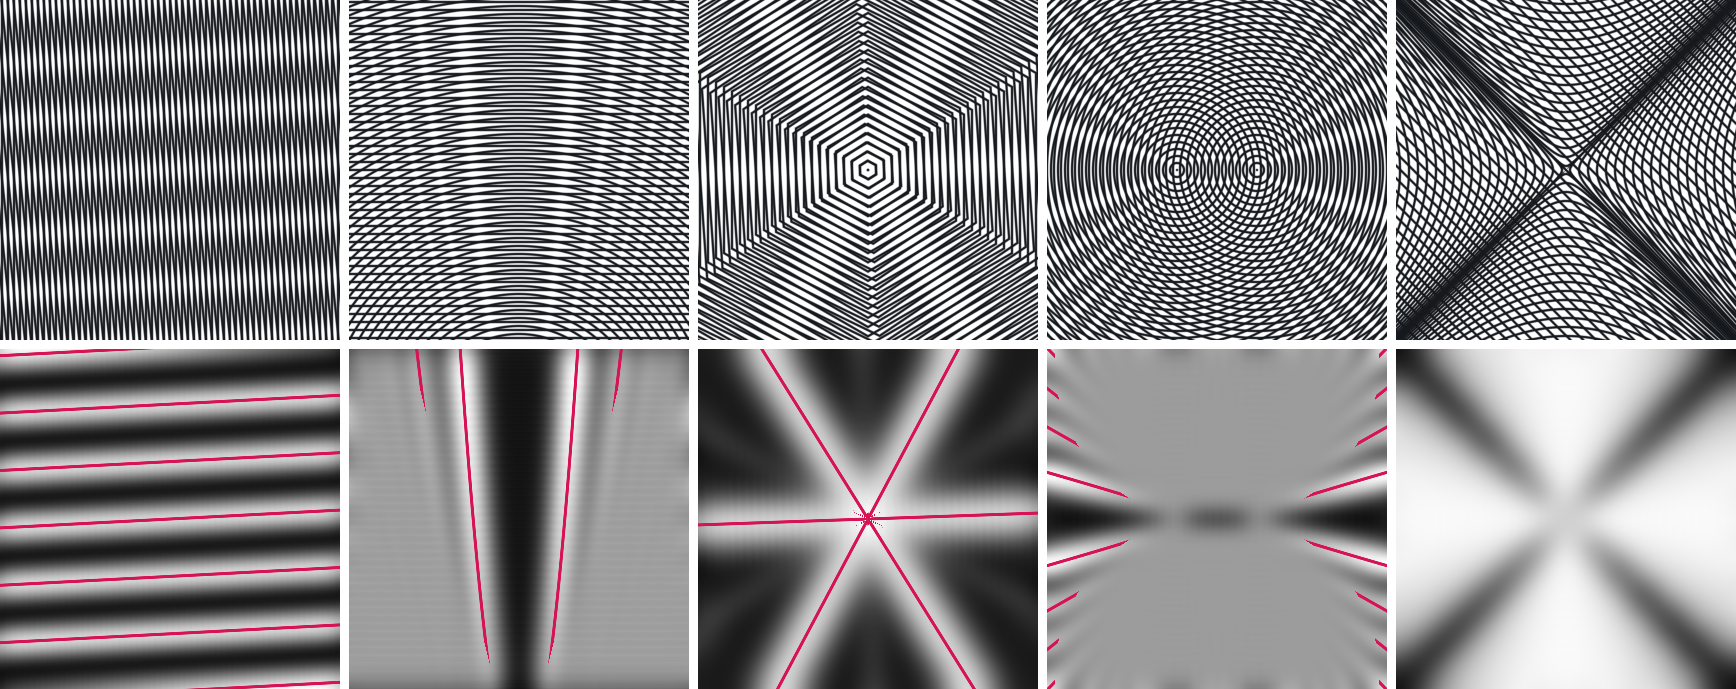
\includegraphics[width=\textwidth]{figures/law-atlas.png}
  \panelrow{0.19576}{0.00530}{%
    (a) two combs,
    (b) circles under lines,
    {(c) hexagons, $4^\circ$},
    {(d) circles, two centers},
    (e) hyperbolae under lines}
  \Description{Two rows of five square panels. The top row shows five moire
  superpositions: two nearly parallel line combs; concentric circles crossed by
  slanted lines; two hexagon families four degrees apart; two circle families with
  displaced centers; and rectangular hyperbolae under slanted lines. The bottom row
  shows the same five frames blurred to gray fringe fields, with crimson curves drawn
  on the light fringes. The crimson curves cover the whole panel in the first, are
  confined to a wedge at one side in the second, radiate as six rays in the third,
  appear only along the top and bottom in the fourth, and in the fifth trace two
  short arcs inside an otherwise refused frame.}
  \caption{\figlead{The law and the criterion, across the catalog.} \emph{Top:} five
  of the pairs measured in Table~\ref{tab:fringe}, rendered from their distance
  fields. \emph{Bottom:} each frame low-passed to its fringe field, with the unit
  level sets of the \emph{winning} character over it in crimson, drawn only where
  the weighted merit $\mu_k\le1/4$ (\S\ref{sec:selection}) and fading out over the
  last tenth of that range, so a curve ending
  is the criterion's edge and not the pixel grid's. Ordered by the fraction of the frame the criterion admits: $\atlasCombs\%$,
  $\atlasCircleLines\%$, $\atlasHex\%$, $\atlasCircles\%$, $\atlasControl\%$.
Column~(b) is masked to a wedge, outside which the circles and the lines cross at
a wide angle; (d) near its two centers, where the superposition is a rosette and
not a fringe field at all. Column~(e) is the instructive one: the first-order
criterion refuses this frame outright (Table~\ref{tab:fringe}'s last row has no
in-regime samples), the bright corridor along the asymptotes belongs to the
hyperbola family alone, and the $\atlasControl\%$ the order-free scan still
admits is a pair of commensurate pockets where a higher-order character locks
onto the hyperbolae, the same stations Figure~\ref{fig:selection}a resolves.
Curves are also suppressed wherever consecutive level
  sets fall closer together than they can be drawn apart: at the center of (c)
  the difference is singular and its level sets crowd without bound, so anything
  drawn there would be speckle rather than a curve. The curves come from the two
  index fields and the mask from their gradients, so the whole bottom row costs two
  gradients per pixel and reads no raster, which is why the tool can tell a user
  that a pair of layers will not interfere before it draws them.}
  \label{fig:lawatlas}
\end{figure*}

\paragraph{Step 4: the hard-edged limit.}
Let $b_i\to0$, so $A_i$ becomes the indicator of
$\{\mathrm{pd}(v,1)\le w_i\}$, an interval of length $2w_i$ per period. Then
$\int_0^1 A_i=2w_i$, and $\int_0^1A_1(v)A_2(v-\Delta)\,\mathrm{d}v$ is the
overlap of two arcs of half-widths $w_1$ and $w_2$ whose centers are
$t=\mathrm{pd}(\Delta,1)$ apart. That overlap is $w_1+w_2-t$ only while the arcs
partially overlap; once one lies inside the other ($t\le|w_1-w_2|$) it saturates
at $2\min(w_1,w_2)$, and once they separate it is zero, so
$\mathrm{overlap}=\min\big(2\min(w_1,w_2),\,\max(0,\,w_1+w_2-t)\big)$. A second
overlap across the far side of the period would need $w_1+w_2>1-t\ge\tfrac12$,
which the theorem's hypothesis $w_1+w_2\le\tfrac12$ excludes; this is where
that hypothesis is used, and without it \eqref{eq:tent} overcounts (the integral
form \eqref{eq:phi} does not). Hence
\begin{equation}
  \Phi(\Delta)=2w_1+2w_2-\min\!\big(2\min(w_1,w_2),\;\max\big(0,\;w_1+w_2-t\big)\big),
\end{equation}
which is \eqref{eq:tent}. It is piecewise linear in $t$, with slope $0$ while one
stroke lies inside the other, slope $1$ while they partially overlap, and slope $0$
after they separate: a tent with a flat floor and a flat top, minimized at
$\Delta\in\Z$ at the value $2\max(w_1,w_2)$ and maximized at $2w_1+2w_2$ wherever
$t\ge w_1+w_2$. Note that the plateau is reached strictly inside the period
whenever $w_1+w_2<\tfrac12$, which is the regime the tool operates in and the
reason thickening strokes eventually stops changing the fringe.

\paragraph{Step 5: the non-constant case, and why the error is first order.}
Suppose now that $D$ varies on $S$; with the gradients constant it is affine
there. In the index variable write $D=D(p)+\mu\,(v-v_p)$, where $\mu$ is the
change in $D$ per unit index, so that
$\lvert\mu\rvert\le\het+O(\het^2)$ by the definition of $\het$ (with equality
when $\nabla D$ is parallel to $u$). Put
$F(v,\Delta)=A_1(v)+A_2(v-\Delta)-A_1(v)A_2(v-\Delta)$, so that
$\Phi(\Delta)=\int_0^1F(v,\Delta)\,\mathrm{d}v$. Averaging over the period and
expanding in $\mu$,
\begin{equation}
  \bar\alpha(p)=\Phi\big(D(p)\big)
  +\mu\int_{-1/2}^{1/2}\!\! (v-v_p)\,\partial_\Delta F\big(v,D(p)\big)\,\mathrm{d}v
  +O(\mu^2).
  \label{eq:appfirst}
\end{equation}
The integral is bounded: $\partial_\Delta F(v,\Delta)=A_2'(v-\Delta)\,(A_1(v)-1)$,
$\lvert v-v_p\rvert\le\tfrac12$ on the period, $\lvert A_1-1\rvert\le1$, and
$\int_0^1\lvert A_2'\rvert\le2$ for the single-bump profile \eqref{eq:appprofile},
so the correction is at most $\lvert\mu\rvert$ in absolute value. Hence
$\bar\alpha(p)=\Phi(D(p))+O(\het)$, as claimed.
\end{proof}

\begin{remark}
The first-order term does not vanish identically. It is odd in
$(v-v_p)$ against a factor that is not even, so no symmetry argument kills it,
and one should expect a genuine $O(\het)$ perturbation of the profile: a
slight asymmetry leaning in the direction the carrier is changing. Its effect
on the \emph{positions} of the extrema depends also on the profile's curvature
there, and on a plateaued extremum the position is not $O(\het)$-stable at all;
the measured statistic is consistent with this: the light fringes of
Table~\ref{tab:fringe} sit at mean index gap $\fringeLight$ from an integer
rather than at $0$, a fraction of the regime bound $\het=1/4$.
\end{remark}

Figure~\ref{fig:lawatlas} is the theorem and its hypothesis drawn together, on five
of the pairs Table~\ref{tab:fringe} measures.

\paragraph{The remaining proofs.} Each bound of \S\ref{sec:inverse} is short and is
proved where it is stated: the drift constant in \S\ref{sec:drift}, the two-sided
envelope as Lemma~\ref{lem:envelope}, the sufficient interval as
Theorem~\ref{thm:window}, the Lipschitz skip as Lemma~\ref{lem:lipschitz}, the
translated-polygon closed form as Proposition~\ref{prop:closed}. The fold law
and its consequences are proved below.

\subsection{The fold law and the reach of closed forms}
\label{app:foldlaw}

\begin{proof}[Proof of Lemma~\ref{lem:foldlaw}]
For a convex body with $C^2$ support function $H_n$, the boundary is
parameterized over contact angles by
$x(u,n)=H_n(u)\,\hat u+H_n'(u)\,\hat u^{\perp}$, with
$\hat u=(\cos u,\sin u)$ and $\hat u^{\perp}=(-\sin u,\cos u)$; this is the
standard support parameterization~\cite{Schneider2014Convex}. Differentiating,
and using $\hat u'=\hat u^{\perp}$, $(\hat u^{\perp})'=-\hat u$,
\begin{equation*}
  \frac{\partial x}{\partial u}=(H_n+H_n'')\,\hat u^{\perp},
  \qquad
  \frac{\partial x}{\partial n}
    =(\partial_nH_n)\,\hat u+(\partial_nH_n')\,\hat u^{\perp},
\end{equation*}
so $\det[\partial_ux,\ \partial_nx]
=(H_n+H_n'')\,(\partial_nH_n)\,\det[\hat u^{\perp},\hat u]
=-(H_n+H_n'')\,\partial_nH_n$. The factor $H_n+H_n''$ is the curvature radius
of the member, nonnegative by convexity, so away from the corner set the
member map is singular --- the family has an envelope, its fold --- exactly
where $\partial_nH_n=0$. Differentiating \eqref{eq:famsupport} in $n$ gives
\eqref{eq:foldlaw}. A polygon's $H$ is piecewise trigonometric with corners
at the vertex directions; the lemma applies on each smooth arc, the one-sided
derivatives at a corner are the two adjacent facets' endpoints (the body's
vertices), and the suprema below are attained there.
\end{proof}

\begin{proof}[Proof of Corollary~\ref{cor:rotation}]
With $\delta=0$, \eqref{eq:foldlaw} reads $sH(w)=\rho_n\theta H'(w)$, i.e.
$\rho_n=s/(\theta\cdot H'(w)/H(w))$, solvable at the smallest gauge radius
$\rho^\star=s/(\theta L)$ with $L=\sup_w|H'/H|$ (the catalog's gauges are
symmetric, so the sup is attained with either sign). For the regular $k$-gon
of unit inradius, $H(u)=\sec(\pi/k)\cos(\tilde u)$ on each arc, where
$\tilde u\in[-\pi/k,\pi/k]$ is the offset from the nearest vertex direction;
$|(\log H)'|=|\tan\tilde u|\le\tan(\pi/k)$, attained at the arc ends. There
$H=1$, $H'=\mp\tan(\pi/k)$, and the fold point
$x=\rho(H\hat u+H'\hat u^{\perp})$ has
$\lVert x\rVert=\rho\sqrt{1+\tan^2(\pi/k)}=\rho\sec(\pi/k)$: the vertex, at
Euclidean radius $R^\star=\rho^\star\sec(\pi/k)=s/(\theta\sin(\pi/k))$. For
the ellipse gauge, $H(u)=\sqrt{a^2\cos^2u+b^2\sin^2u}$; writing
$A=(a^2+b^2)/2$, $B=(a^2-b^2)/2$, we have $H^2=A+B\cos2u$ and
$(\log H)'=-B\sin2u/H^2$, maximized at $\cos2u^\star=-B/A$ with value
$B/\sqrt{A^2-B^2}=(a^2-b^2)/2ab=L$. At $u^\star$, $H^2=a^2b^2/A$ and
$H'^2=B^2/A$, so
$\lVert x\rVert=\rho\sqrt{H^2+H'^2}=\rho\sqrt{(a^2b^2+B^2)/A}=\rho\sqrt{A}$,
since $a^2b^2+B^2=A^2$: the stated $R^\star=\rho^\star\sqrt{(a^2+b^2)/2}$.
Finally $L=0$ iff $H'\equiv0$ iff $H$ is constant iff $K$ is a centered
disc, so the circle is the unique rotation-immune gauge.
\end{proof}

\begin{proof}[Proof of Corollary~\ref{cor:mach}]
With $\theta=0$, $\partial_nH_n(u)=sH(u)+\langle\delta,\hat u\rangle$, which
is negative somewhere iff
$\sup_u\langle-\delta,\hat u\rangle/H(u)>s$. That supremum is the gauge:
$x\in tK$ iff $\langle x,\hat u\rangle\le tH(u)$ for all $u$, so
$\sup_u\langle x,\hat u\rangle/H(u)=\rad(x)$, and the fold condition is
$\rad(-\delta)>s$, uniform in $n$ (hence ``immediately''). At a critical
angle $u^\star$ the envelope points
$x(u^\star,n)=H_n(u^\star)\hat u^\star+H_n'(u^\star)\hat u^{\star\perp}$ are
affine in $n$: straight wake lines. For circles ($H\equiv1$) the critical
directions are the unit vectors $\nu$ with
$\langle\delta,\nu\rangle=-s$, and
$\langle x,\nu\rangle=H_n(u^\star)=ns+\varphi+n\langle\delta,\nu\rangle=\varphi$:
the tangent pair. With rotation, $c(n)=\Rot{n\theta}(n\delta)$ gives
$c'(n)=\Rot{n\theta}\delta+n\theta\,\Rot{n\theta+\pi/2}\delta$, two orthogonal
components of lengths $\lVert\delta\rVert$ and $n\theta\lVert\delta\rVert$,
so $\lVert c'(n)\rVert=\lVert\delta\rVert\sqrt{1+n^2\theta^2}$, and for
circles the condition $\lVert c'(n)\rVert>s$ first holds at
$n^\star=\sqrt{(s/\lVert\delta\rVert)^2-1}/\theta$.
\end{proof}

\begin{proof}[Proof of Proposition~\ref{prop:untwist}]
Rational case: with $\theta=2\pi a/b$ and $n=j+bk$,
$n\theta\equiv j\theta\pmod{2\pi}$, so on the class the pulled-back point is
$\Rot{-j\theta}p-n\delta$: a fixed rotation of $p$ minus an affine walk. The
residual is a convex gauge of an affine path, hence convex in $n$ on the
class; for the circle gauge,
$\lVert\Rot{-j\theta}p-n\delta\rVert=\lVert p-n\Rot{j\theta}\delta\rVert$,
and squaring the incidence gives one quadratic per class. The frames
$\{n\theta\bmod2\pi\}$ form a finite set iff $\theta/2\pi\in\Q$ (a subgroup
of the circle is finite or dense), so no such split exists otherwise.

Transcendence: suppose the interpolated incidence
$I=\{(p,\nu):\lVert p-c(\nu)\rVert=\nu s+\varphi\}$ were semialgebraic for
some $\theta\neq0$. Each slice $I_\nu$ is a circle of positive radius, and
the center of a circle is first-order definable from the circle over the
real field, so $\nu\mapsto c(\nu)$ would be a semialgebraic function; its
first coordinate $f(\nu)=\nu\lVert\delta\rVert\cos(\nu\theta+\beta)$ would
satisfy $P(\nu,f(\nu))\equiv0$ for some nonzero polynomial
$P(\nu,y)=\sum_{j\le d}q_j(\nu)y^j$ with $q_d\not\equiv0$. Extend to complex
$\nu=it$, $t\to\infty$: $|\cos(it\theta+\beta)|$ grows like
$e^{\theta t}/2$, so the term $q_j(\nu)f(\nu)^j$ grows like
$e^{j\theta t}$ times a polynomial in $t$. The orders are distinct, so the
identity forces $q_d\equiv0$, a contradiction. (For a polygon or ellipse
gauge the same argument runs through the frame angle, definable from a slice
by its vertex or axis directions.)
\end{proof}

\paragraph{Group families never fold.} The claim of \S\ref{sec:taxonomy}:
if $\gamma_0$ crosses each orbit of the flow $\{g^t\}$ exactly once,
transversally, then $(u,t)\mapsto g^t(\gamma_0(u))$ is a bijection onto the
swept region with everywhere-invertible differential (transversality is
preserved because each $g^t$ is a diffeomorphism), so the family
$\{g^n\gamma_0\}$ is a foliation and the index --- the $t$-component of the
inverse --- is a submersion: no envelope can form. A rotational flow's clock
gains its period on each circuit of the fixed point, and the gain counts the
members a circuit crosses, which is the winding rung's quantized charge;
flows without a rotational part have proper orbits and a single-valued
clock.
